% $Id: introduction.tex 34630 2013-04-29 22:53:51Z roldeman $

\section{Optimising the $\alpha_T$ analysis for Run 2 data}
\label{sec:analysisOptimisation}

The major change with Run~2 of the LHC is the increase in energy to 13~TeV and instantaneous luminosity, to peak at $1.6\times10^{34}$~cm$^{-2}$s$^{-1}$, more than twice the peak of $7.7\times10^{33}$~cm$^{-2}$s$^{-1}$ reached in Run~1 \cite{LHCLuminosityIPAC13}. These two factors result in an increase in the number of simultaneous collisions per event and an increase in cross section for all SM processes. However, for SUSY particles outside the reach of Run~1 analyses, the relative increase in cross section increase should be greater than that for the backgrounds. It is therefore necessary to optimise the analysis to take account of the change in conditions. Some of the optimisations and alterations are discussed in this section, having been studied with $13$~TeV Monte Carlo simulation.
\\\\
Events with a single hard jet and missing energy in their final state are particularly sensitive to the pair production of heavy invisible particles. They usually occur when the invisible system is produced in conjunction with initial or final state radiation from one of the colliding partons. To increase sensitivity to events with this topology, only the lead jet is required to have $p_T>100$~GeV, whereas in the Run~1 analysis this was required of the second leading jet. These extra results are added to an asymmetric jet bin, and have been seen to increase sensitivity to SUSY models with a compressed mass spectrum as well as generic models of dark matter pair production. The increase in yields for a compressed SUSY model by allowing a second jet with $p_T<100$~GeV is evident in Fig.~\ref{fig:asymMotivation}.
\\\\
\begin{figure}[h!]
  \centering
  \subfigure[Second jet $p_T$ for $200$~GeV$<H_T<250$~GeV, $\alpha_T>0.65$]{
    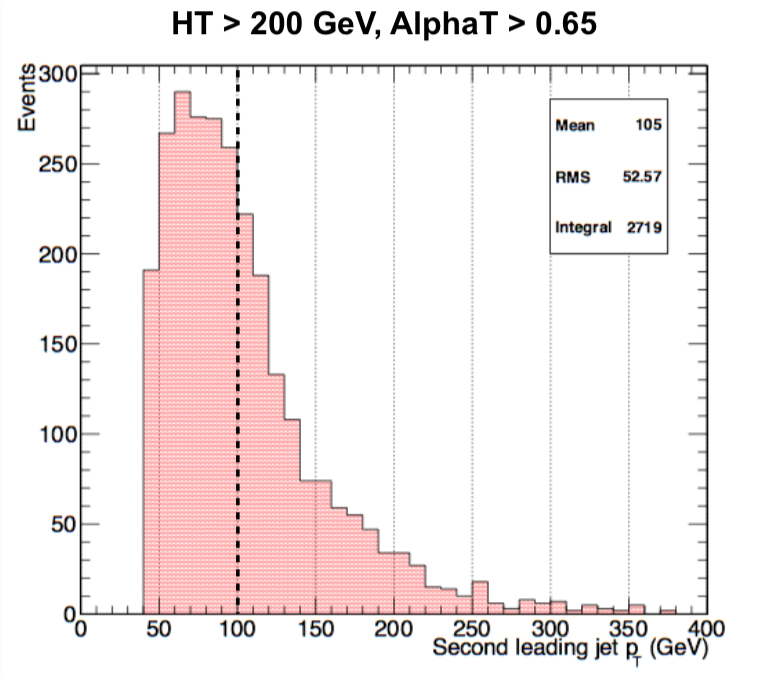
\includegraphics[width=0.5\textwidth]{secondJetPtlowHT}
  }~~
  \subfigure[Second jet $p_T$ for $400$~GeV$<H_T>500$~GeV, $\alpha_T>0.52$]{
    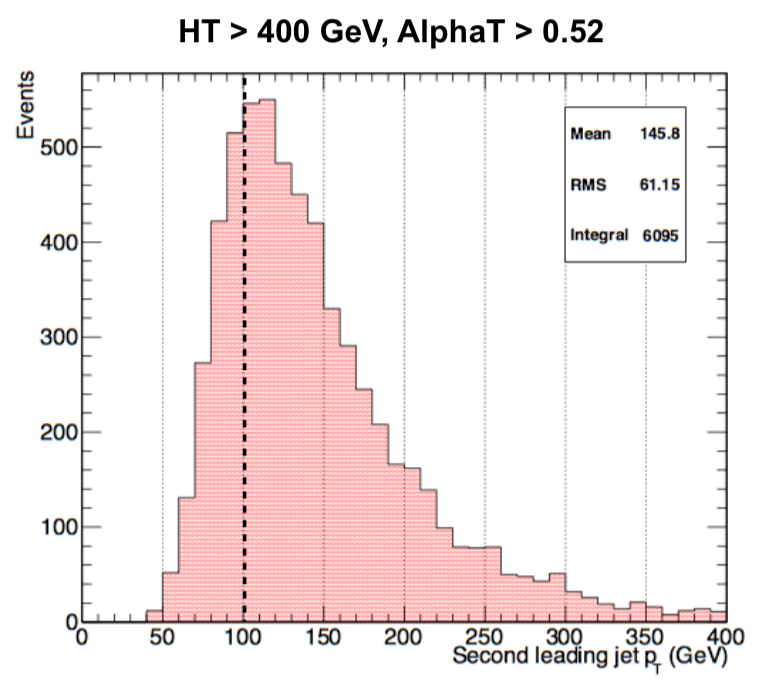
\includegraphics[width=0.5\textwidth]{secondJetPthigherHT}
  }
  \\
  \caption{\label{fig:asymMotivation} The second leading jet $p_T$ for different
  cases of $H_T$ after a baseline signal selection: $N_{jet}\geq2$, lead jet
  $E_T>100\gev$, lepton vetoes. Made with the T2tt ($m_{STOP}=425$~GeV, $m_{LSP}=325$~GeV) simplified model sample.}
\end{figure}

\noindent As the collaboration prepares for Run~2 data taking, the reconstruction algorithms discussed in Sec.~\ref{analysisFw} are developed. As these developments are intended improve overall performance, it is necessary to study the effect of the changes on the $\alpha_T$ analysis and choose the desired parameters for the new algorithms. This also ensures the different analyses in CMS are using consistent object definitions, allowing easy result comparison. The jets we use in the analysis, for example, now utilise tracking information to improve the energy resolution over just the calorimeter information used in Run~1~\cite{ParticleFlow}. Additionally, a new muon reconstruction algorithm improves the efficiency of muon identification but doesn't increase the misidentification rate, allowing a reduction in the W~+~jets and $t\bar{t}$ SM backgrounds. 
\\\\
One additional proposal was a slight change in the lepton isolation algorithm to increase the efficiency of boosted leptons, particularly those produced as the decay products of top quarks. Rather than using a fixed cone around the lepton, the cone size, $R$, was decreased in size according to:
\begin{equation}
R =
  \begin{cases}
    0.2       & p_{T,lep} \leq 50\textrm{GeV}\\
    \frac{10\textrm{GeV}}{p_T,lep}       & 50\textrm{GeV}\geq p_{T,lep} \geq 200\textrm{GeV}\\
    0.05     &  p_{T,lep} \geq 200\textrm{GeV}\\
  \end{cases}
\end{equation}
The result of using this method of isolation on the $\alpha_T$ analysis was checked by running the full analysis with and without the new ``mini isolation'' method. The ratio of the upper limits set on the cross section of a variety of SUSY models can be seen in Table~\ref{tab:miniIsoResult}. In most cases there is an improvement (a decrease in the cross section of the SUSY model that can be excluded). This is most likely due to the improved reduction in $t\bar{t}$ background. However, in the T1tttt model four tops are produced in the final state. By more accurately identifying the leptons in the decay products of these tops, the events move from an apparent hadronic final state to a leptonic one. It is assumed the loss in sensitivity in the $\alpha_T$ analysis will be picked up by a leptonic SUSY analysis.
\\\\
\begin{table}[h!]
  \caption{Changes to sensitivity of various benchmark SUSY models with the new mini isolation algorithm \label{tab:miniIsoResult}}
  \centering
  \footnotesize
  \begin{tabular}{ lcc }
    \hline
    \hline
    SUSY Model     & $\frac{\textrm{mini isolation upper limit on cross section}}{\textrm{normal isolation upper limit on cross section}}$\\ 
    \hline                                                                     
    T1bbbb $m_{\tilde{g}}=1500$~GeV $m_{LSP}=100$~GeV     & 0.95    \\  %& 0.505         \\
    T1tttt $m_{\tilde{g}}=1200$~GeV $m_{LSP}=800$~GeV      & 1.10    \\  %& 0.505         \\
    T2qq $m_{\tilde{t}}=600$~GeV $m_{LSP}=550$~GeV      & 0.97    \\  %& 0.505         \\
    T2tt $m_{\tilde{t}}=500$~GeV $m_{LSP}=325$~GeV       & 0.96    \\  %& 0.505         \\
    \hline
    \hline
  \end{tabular}
\end{table}

\noindent An additional improvement to the analysis is the categorisation of events based on their $\cancel{H_T}$. As SUSY production results in high values of this variable, the signal to background ratio significantly increases at high values of $\cancel{H_T}$. However, the $\alpha_T$ analysis relies on lepton and photon control samples to estimate the SM background in all the analysis bins. This reduces the reliance on the simulation of events with high $\cancel{E_T}$, which isn't well enough understood. There is therefore a limit to how high the bins of $\cancel{H_T}$ can extend, as the control samples must still have some events within these bins. In Run~1 single muon, double muon and single photon control samples were utilised. Single electron and double electron samples, analogous to the muon control samples, are now being introduced to increase the number of events available for background estimation and systematic error determination. Studies on simulation have shown that, with a tight enough requirement on the parameters of the electron identification algorithm, the electron control samples do not suffer from QCD contamination. They therefore effectively double the statistics available in the lepton control samples.
